% Chapter 3: State of the Art

\chapter{Estado del Arte} % Main chapter title

\label{Chapter3} % For referencing this chapter elsewhere, use \ref{Chapter2}

%----------------------------------------------------------------------------------------

 \section{Java}

 \keyword{Java} es un lenguaje de programación de propósito general, orientado a objetos y concurrente. Originalmente fue desarrollado por James Gosling, Bill Joy y Guy Steele para Sun Microsystems en 1996 y fue adquirido por Oracle en 2010.

 Fue diseñado para que los desarrolladores escribiesen una única vez su programa y pudieran ejecutarlo en cualquier máquina sin necesitar recompilarlo.
 Esto es posible debido a que las aplicaciones Java son compiladas a \emph{bytecode} que luego es ejecutado en una \keyword{Java Virtual Machine (JVM)}, sin importar la arquitectura de la máquina. \emph{\parencite{Reference13}}

 \begin{figure}[ht]
   \centering
   
\includegraphics[scale=0.4]{Figures/JavaLogo}
   \decoRule
   \caption[Java (Logo)]{Logo de Java} \emph{\parencite{Reference6}}
   \label{fig:JavaLogo}
 \end{figure}

 %----------------------------------------------------------------------------------------

 \section{Android}

 \keyword{Android} es un sistema operativo propiedad de Google, basado en el \emph{kernel} de Linux. Está diseñado principalmente para dispositivos táctiles, como \emph{smartphones} y \emph{tablets}.

 \keyword{Android} es compatible con las librerías de Java, por lo que la mayoría de las aplicaciones están escritas en ese lenguaje.
 Desde la versión 4.4 de Android, se utiliza \keyword{Android Runtime} (\keyword{ART}) como entorno de ejecución\footnote{En versiones anteriores se utilizaba Dalvik y su máquina virtual.},
 el cual compila completamente el \emph{bytecode} a código máquina durante la instalación de la aplicación. \emph{\parencite{Reference7}}

 \begin{figure}[ht]
   \centering
   
\includegraphics[scale=0.05]{Figures/AndroidLogo}
   \decoRule
   \caption[Android (Logo)]{Logo de Android} \emph{\parencite{Reference7}}
   \label{fig:AndroidLogo}
 \end{figure}

 %----------------------------------------------------------------------------------------

 \section{Bouncy Castle}

 \keyword{Bouncy Castle (BC)} es una colección de APIs utilizados en criptografía.
 Estas APIs, entre otras cosas, proporcionan los siguientes servicios:
 \begin{itemize}
 \item Una API criptográfica \emph{ligera} para Java y C\#.
 \item Un proveedor para Java Cryptography Extension (JCE)\footnote{JCE implementa encriptación, generación y protocolos de establecimiento de claves y algoritmos MAC.} y para Java Cryptography Architecture (JCA).
 \end{itemize}

 Todas las APIs de BC están mantenidas por una organización caritativa australiana, conocida como \keyword{The Legion of the Bouncy Castle}. \emph{\parencite{Reference4}}

 \begin{figure}[ht]
   \centering
   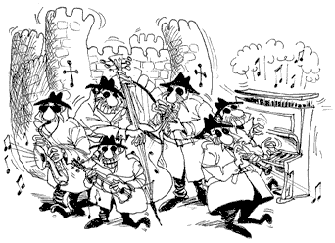
\includegraphics[scale=0.5]{Figures/BouncyCastle}
   \decoRule
   \caption[Legion of the Bouncy Castle]{The Legion of the Bouncy Castle, creadores de Bouncy Castle} \emph{\parencite{Reference4}}
   \label{fig:BouncyCastle}
 \end{figure}

 %----------------------------------------------------------------------------------------

 \section{Padding}

 \keyword{Padding} es el nombre que recibe la técnica que permite en criptografía por bloques expandir el último bloque del mensaje hasta lograr un tamaño deseado.

 Es muy común que, en la criptografía por bloques, los fragmentos que encriptamos no tengan la longitud que queremos para nuestro sistema. Para solucionar esto existen multitud de técnicas de \keyword{padding},
 desde agregar al final del bloque un byte con un cierto valor, hasta simplemente rellenar con ceros.

 El requisito indispensable que debe cubrir cualquier técnica de padding es que debe permitir al destinatario diferenciar los bytes del mensaje original de los byte de relleno. \emph{\parencite{Reference8}}

 %----------------------------------------------------------------------------------------

 \section{Criptografía de clave pública}

 Uno de los problemas que tiene la \keyword{criptografía de clave simétrica} es que necesita de un medio seguro para compartir la clave de cifrado entre los componentes de la comunicación.
 La \keyword{criptografía de clave pública} soluciona este problema al no ser necesario crear un canal seguro para el establecimiento de la clave, ya que para este modelo se hace uso de un par de claves: una \emph{pública} y otra \emph{privada}.

 La esencia de este algoritmo radica en que un mensaje cifrado con una clave pública solo puede ser descifrado con su homóloga privada, y viceversa.
 De esta manera podemos, tal como su propio nombre indica, difundir públicamente nuestra clave \emph{pública} mientras mantenemos oculta la \emph{privada}.

 Si lo que queremos es \emph{confidencialidad} durante la comunicación, entonces encriptaremos el contenido del mensaje con la clave pública del destinatario, de forma que solo él podrá descifrarlo (Figura~\ref{fig:PublicKeyEncryption}).

 Por otra parte, también nos interesa que cuando alguien reciba nuestro mensaje pueda estar seguro de que realmente es nuestro.
 Para lograr esto, lo que hacemos es cifrar un resumen del mensaje (\emph{hash}) con nuestra clave privada.
 De esta forma, cuando alguien lo descifre con nuestra clave pública y compruebe el resumen, podrá estar seguro de que proviene de nosotros.\footnote{Es, en esencia, el fundamento sobre el que se basa la firma digital.}
 Así conseguimos preservar la \emph{integridad} y la \emph{autentificación} del mensaje, dos parámetros muy importantes a tener en cuenta en seguridad. \emph{\parencite{Reference14}}

 \begin{figure}[ht]
   \centering
   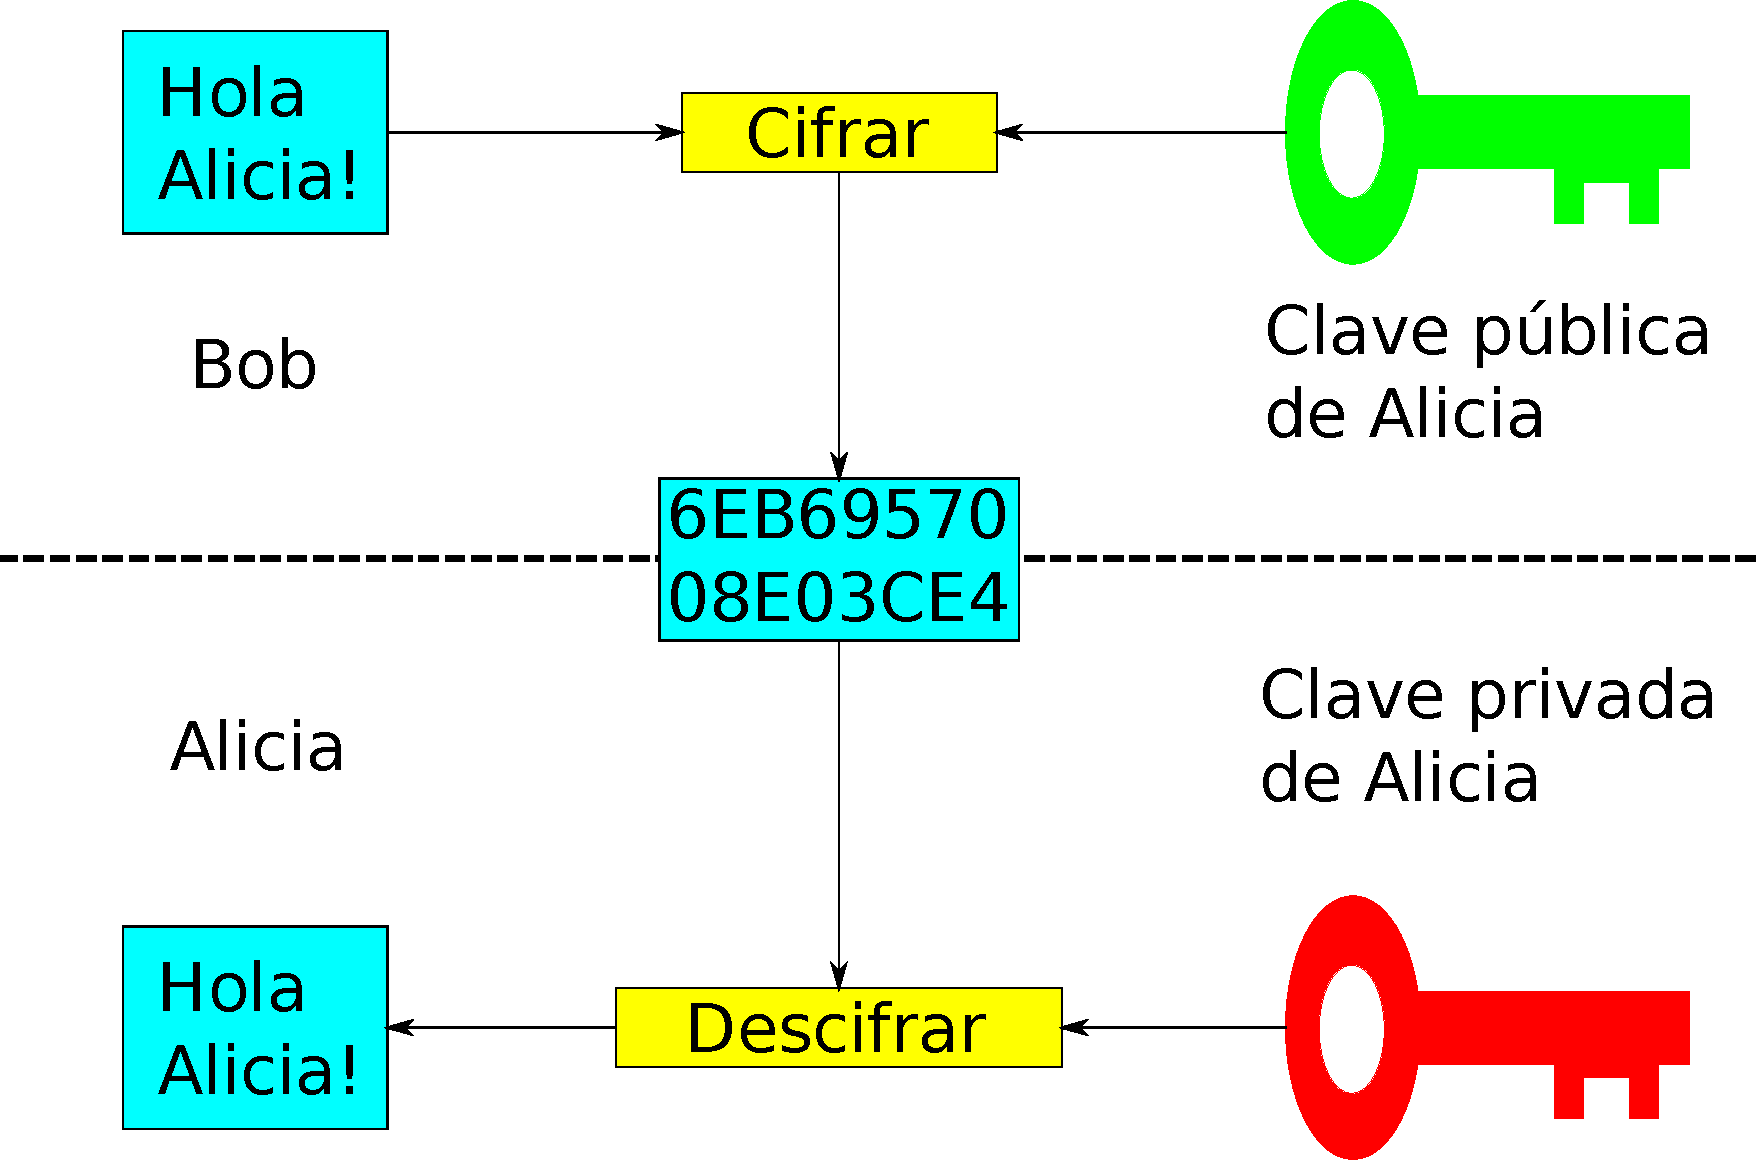
\includegraphics[scale=0.5]{Figures/PublicKeyEncryption}
   \decoRule
   \caption[Cifrado de clave pública (Esquema)]{Esquema general del cifrado de clave pública} \emph{\parencite{Reference5}}
   \label{fig:PublicKeyEncryption}
 \end{figure}

 %----------------------------------------------------------------------------------------

 \section{RSA}

 Uno de los primeros algoritmos de criptografía pública (y el más utilizado hoy) es \keyword{RSA} (\keyword{Rivest–Shamir–Adleman})\footnote{RSA debe su nombre a sus creadores: Ron Rivest, Adi Shamir y Leonard Adleman.}.
 Una de sus características más distintivas es el uso de números primos y la factorización de sus productos en la generación de las claves y en la encriptación/desencriptación de los mensajes (\emph{factoring problem}).

 \keyword{RSA} no es el más rápido de los algoritmos de criptografía que existen actualmente. Por ello, muchas veces se recurre a su uso en conjunto con otros algoritmos de criptografía simétrica, como \keyword{AES}. \emph{\parencite{Reference9}}

 \subsection{Clave pública RSA}

 Dentro del conjunto del par de claves \keyword{RSA}, la \emph{pública} es la que se distribuye públicamente para que cualquiera que quisiera comunicarse con nosotros pudiera hacerlo de manera confidencial.
 Este tipo de claves consta de dos elementos:
 \begin{itemize}
 \item \keyword{n} -- el módulo RSA, un entero positivo.
 \item \keyword{e} -- el exponente público RSA, otro entero positivo.
 \end{itemize}

 Lo primero que se debe hacer para generar la clave \emph{pública} es seleccionar de manera aleatoria dos números primos impares distintos, lo suficientemente grandes como para que sea computacionalmente inviable su descubrimiento por parte de un atacante.
 Una vez encontrados, el módulo \keyword{n} de la clave \emph{pública} será el producto de estos dos números primos.\footnote{Por convención, se denotan como \emph{p} y \emph{q}.}
 \[ n = p \boldsymbol{\cdot} q \]

 Ahora que tenemos el módulo de la clave definido, es hora de generar un exponente público \keyword{e} adecuado.
 Para ello, haremos uso de la función de Carmichael\footnote{La función que se muestra solo es válida cuando n es el producto de dos números primos impares y distintos.}, la cual tiene la siguiente forma:
 \[ \lambda(n) = mcm\footnote{Mínimo común múltiplo.}(p - 1, q - 1) \]
 El exponente público \keyword{e} será aquel número entero comprendido entre 3 y (\keyword{n} - 1) que satisfaga:
 \[ MCD\footnote{Máximo común divisor.}(e, \lambda(n)) = 1 \] \emph{\parencite{Reference10}}

 \subsection{Clave privada RSA}

 La clave \emph{privada} es la que mantenemos oculta. Aunque existen varios modelos, generalmente consta de dos elementos:
 \begin{itemize}
 \item \keyword{n} -- el módulo RSA, un entero positivo (Debe ser el mismo que el de la clave \emph{pública}).
 \item \keyword{d} -- el exponente privado RSA, un entero positivo.
 \end{itemize}

 Para calcular el exponente privado \keyword{d} deberemos elegir un entero positivo menor que \keyword{n}, que además cumpla:
 \[ e \boldsymbol{\cdot} d \equiv 1 \Mod{\lambda(n)} \]
 , donde \keyword{e} será el correspondiente exponente público. \emph{\parencite{Reference11}}

 \subsection{Evaluación de la función RSA}

 Lo primero que debemos hacer es conseguir una representación de nuestro mensaje como un número entero, comprendido entre 0 y (\keyword{n} - 1).

 Vamos a suponer que este mensaje queremos enviárselo a alguien cuya clave pública es (\emph{e, n}).
 Si nuestro mensaje (recordemos que ahora es un entero) es \emph{M}, para obtener el mensaje cifrado, aplicaremos la siguiente operación:
 \[ C \equiv E(M) \equiv M^e \Mod{n} \]
 El entero \emph{C} será del mismo tamaño que \emph{M} y representará al mensaje cifrado.

 Si ahora el destinatario quisiera descifrar el mensaje, solo tendría que revertir la operación con su clave privada (\emph{d, n}) de la siguiente manera:
 \[ M \equiv D(C) \equiv C^d \Mod{n} \]
 De esta manera, recuperaría el mensaje original.\footnote{Para cifrar con una clave privada y descifrar con una pública se hacen las mismas operaciones, cambiando e y d donde corresponda.} \emph{\parencite{Reference12}}

 %----------------------------------------------------------------------------------------

 \section{RSASSA-PSS}

 Antes hablamos de la necesidad de preservar la \emph{integridad} y la \emph{autentificación} en las comunicaciones.
 \keyword{RSASSA-PSS} es un algoritmo de firma digital que sirve precisamente para ello.
 Combina lo visto de RSA con un método de codificación llamado Probabilistic Signature Scheme (PSS).
 \footnote{Las siglas SSA corresponden a Signature Scheme with Appendix, lo que quiere decir que la firma va añadida al final del mensaje o junto a él.}

 \subsection{Probabilistic Signature Scheme (PSS)}

 \keyword{PSS} es un método de codificación\footnote{Un método de codificación es una operación que permite convertir un carácter de un determinado conjunto en un símbolo de otro sistema de representación.}
 desarrollado por Mihir Bellare y Phillip Rogaway, los cuales buscaban mejorar los métodos que existían.
 Para ello, incluyeron en su esquema el uso de una \emph{salt},\footnote{Bits aleatorios.} lo cual haría más seguro el algoritmo frente a intentos de romperlo. \emph{\parencite{Reference15}}

 \begin{figure}[ht]
   \centering
   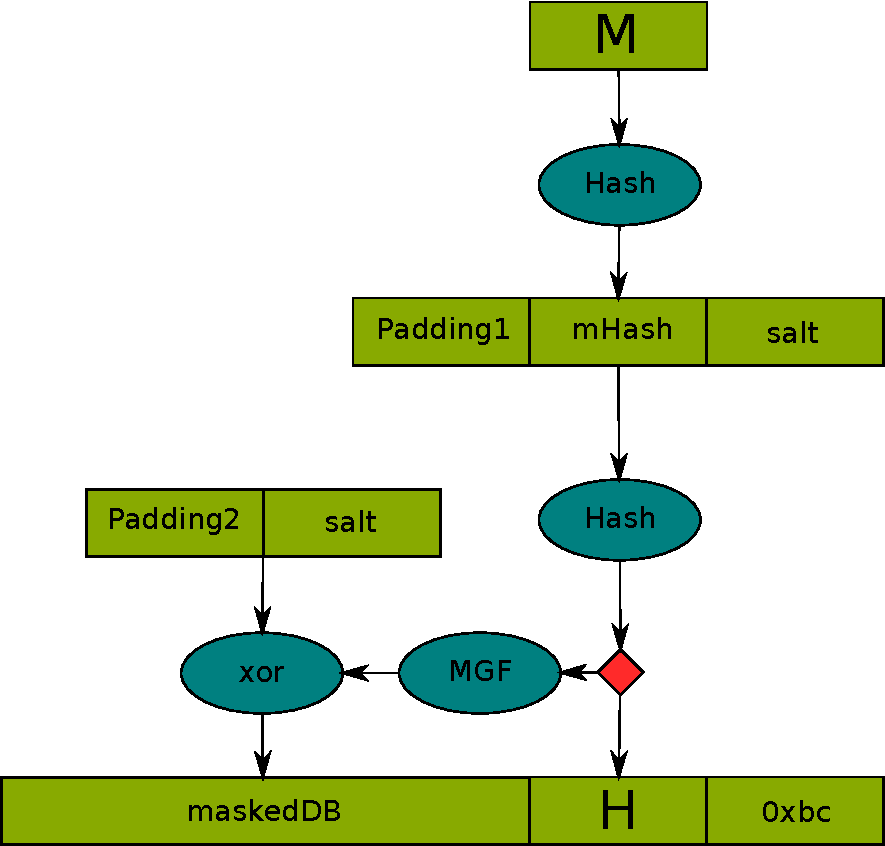
\includegraphics[scale=2.0]{Figures/PSS}
   \decoRule
   \caption[PSS (Esquema)]{PSS de acuerdo a PKCS \#1 V2.2 / RFC 8017} \emph{\parencite{Reference16}}
   \label{fig:PSS}
 \end{figure}

 Como vemos en la Figura~\ref{fig:PSS}, \keyword{PSS} genera un resumen (\emph{hash}) del mensaje.
 Este resumen se vuelve a pasar de nuevo por una función \emph{hash}\footnote{Las dos funciones \emph{hash} que se usan en el esquema deben ser la misma.} junto a un \emph{padding}\footnote{El primer \emph{padding} estará formado por 8 bytes con valor \emph{0x00}.} y la \emph{salt} tal como muestra la figura.

 El resultado de esta operación será la segunda de 3 piezas que conformarán nuestro mensaje codificado y la denotaremos como \keyword{H}.
 Para la primera (\emph{maskedDB}), generaremos una máscara\footnote{Una máscara es muy parecida a una \emph{hash}. Mientras la segunda tiene un tamaño determinado, una máscara puede tomar distintos tamaños según la necesidad.} de \keyword{H} y haremos una operación \emph{xor} con ella y la salt (junto a otro \emph{padding}).\footnote{Este \emph{padding} está formado por una cantidad variable de bytes con valor \emph{0x00}, teniendo al final un byte de valor \emph{0x01}.}

 Ahora solo nos quedará añadir al final de nuestra salida un byte con valor \emph{0xbc} y ya habremos acabado. \emph{\parencite{Reference17}}

 %----------------------------------------------------------------------------------------

 \section{Criptografía de clave simétrica}

 %----------------------------------------------------------------------------------------

 \section{Cifrado de bloques}

 %----------------------------------------------------------------------------------------

 \section{CBC}

 %----------------------------------------------------------------------------------------

 \section{AES}

 %----------------------------------------------------------------------------------------

 \section{HTTP}
